% Gemini beamerposter source
% Theme: https://github.com/anishathalye/gemini
% !TeX program = lualatex
% !BIB program = bibtex
\documentclass[final]{beamer}

\usepackage[size=custom,width=91.44,height=60.96,scale=0.80]{beamerposter}
\usetheme{gemini}
\usecolortheme{gemini}

\usepackage{booktabs}
\usepackage{graphicx}
\usepackage{tabularx}
\usepackage{array}
\usepackage{ragged2e}
\usepackage{microtype}
\usepackage{iftex}
\usepackage{url}
\usepackage{xcolor}

\ifPDFTeX
\else
  \usepackage{unicode-math}
  \setmathfont{Latin Modern Math}
\fi

\graphicspath{{../results/analysis/}}

% ====================
% Layout
% ====================

\newlength{\sepwidth}
\newlength{\colwidth}
\setlength{\sepwidth}{0.017\paperwidth}
\setlength{\colwidth}{0.310666\paperwidth}
\newcommand{\separatorcolumn}{\begin{column}{\sepwidth}\end{column}}

\setbeamerfont{block title}{size=\Large,series=\bfseries}
\setbeamerfont{block body}{size=\normalsize}
\setbeamerfont{heading}{size=\normalsize,series=\bfseries}
\setbeamerfont{caption}{size=\footnotesize}
\setlength{\tabcolsep}{3.5pt}
\renewcommand{\arraystretch}{1.08}

\newcommand{\tightcaption}[1]{%
  \vspace{-0.7ex}%
  \par\noindent{\footnotesize\RaggedRight\textbf{Figure.} #1\par}%
  \vspace{0.6ex}%
}

\newcommand{\resultnote}[2]{%
  \par\noindent{\footnotesize\RaggedRight\textbf{#1.} #2\par}%
}

\newcommand{\shortcite}[1]{\raisebox{0.65ex}{\scriptsize\cite{#1}}}
\newcommand{\dora}{\textcolor{NvidiaGreenDark}{\textbf{DoRA}}}
\newcommand{\lora}{\textcolor{MicrosoftBlue}{\textbf{LoRA}}}

% ====================
% Title
% ====================

\title{Reproducing DoRA for Commonsense Reasoning with Student-Scale Compute}
\author{Ian Holloway \and Younghyun Jung \and Swathi Saravana Selvam \and Shashwat Modi}
\institute{Cornell University \samelineand CS 5782 / CS 4782 Intro to Deep Learning}

\footercontent{Llama-2-7B commonsense reasoning reproduction \hfill \dora{} = Nvidia green, \lora{} = Microsoft blue \hfill 36 in x 24 in}

\begin{document}

\begin{frame}[t]
\begin{columns}[t]
\separatorcolumn

% ====================
% Column 1
% ====================

\begin{column}{\colwidth}

\begin{exampleblock}{Motivation \& Paper Idea}
Full fine-tuning large language models is expensive in memory, storage, and training time. \lora{} reduces this cost by training low-rank adapter updates while freezing the base model, but the low-rank update alone may limit how pretrained weights can change.\shortcite{hu2022lora}

\heading{DoRA}
\begin{itemize}
  \item \dora{} decomposes pretrained weights into \textbf{magnitude} and \textbf{direction}.\shortcite{liu2024dora}
  \item Direction receives a \lora{}-style low-rank update; magnitude is learned separately.
  \item The paper reports improved accuracy over \lora{} across multiple tasks.
\end{itemize}

\heading{Project goal}
\begin{itemize}
  \item Reproduce the paper's LLaMA2-7B commonsense reasoning trend.
  \item Test whether \dora{} helps most in attention layers, MLP layers, or only when applied broadly.
\end{itemize}
\end{exampleblock}

\begin{block}{Methodology}
\heading{Model, data, and metrics}
\begin{itemize}
  \item Base model: \texttt{meta-llama/Llama-2-7b-hf}.
  \item Training data: \texttt{commonsense\_15k.json}, a student-scale commonsense subset.
  \item Evaluation: BoolQ, PIQA, Social IQA, HellaSwag, WinoGrande, ARC-Easy, ARC-Challenge, OpenBookQA.
  \item Metrics: per-task accuracy and macro-average accuracy across all eight tasks.
\end{itemize}

\heading{Implementation}
\begin{itemize}
  \item Repo-owned PyTorch \lora{} and \dora{} adapter layers.
  \item Hugging Face \texttt{transformers} model/tokenizer loading and generation.
  \item Frozen base model, adapter-only checkpoints, 3 epochs, cutoff length 256.
  \item Colab-focused 4-bit NF4 runtime presets for T4, L4, and A100 GPUs.
\end{itemize}
\end{block}

\begin{block}{Independent Scope Ablation}
\small
\begin{tabularx}{\linewidth}{>{\bfseries}l X X}
\toprule
Scope & Target modules & Purpose \\
\midrule
Full & \texttt{q,k,v,up,down} projections & Paper-level reproduction \\
Attention only & \texttt{q,k,v} projections & Test routing/context layers \\
MLP only & \texttt{up,down} projections & Test feed-forward layers \\
\bottomrule
\end{tabularx}
\normalsize

\vspace{0.8ex}
\resultnote{Design}{Each scope compares matched \lora{} and \dora{} adapters under the same evaluation pipeline.}
\end{block}

\end{column}

\separatorcolumn

% ====================
% Column 2
% ====================

\begin{column}{\colwidth}

\begin{alertblock}{Headline Result}
\begin{columns}[T,totalwidth=\linewidth]
\begin{column}{0.24\linewidth}
\centering{\Huge\bfseries 77.41\%}\par{\footnotesize Full \lora{} macro}
\end{column}
\begin{column}{0.24\linewidth}
\centering{\Huge\bfseries 79.20\%}\par{\footnotesize Full \dora{} macro}
\end{column}
\begin{column}{0.24\linewidth}
\centering{\Huge\bfseries +1.79}\par{\footnotesize accuracy points}
\end{column}
\begin{column}{0.24\linewidth}
\centering{\Huge\bfseries 6/1/1}\par{\footnotesize wins/ties/losses}
\end{column}
\end{columns}
\vspace{0.8ex}
\centering{\footnotesize Full-scope \dora{} reproduced the paper's qualitative improvement over \lora{} under our student-scale setup.\par}
\end{alertblock}

\begin{block}{Macro Accuracy by Adapter Scope}
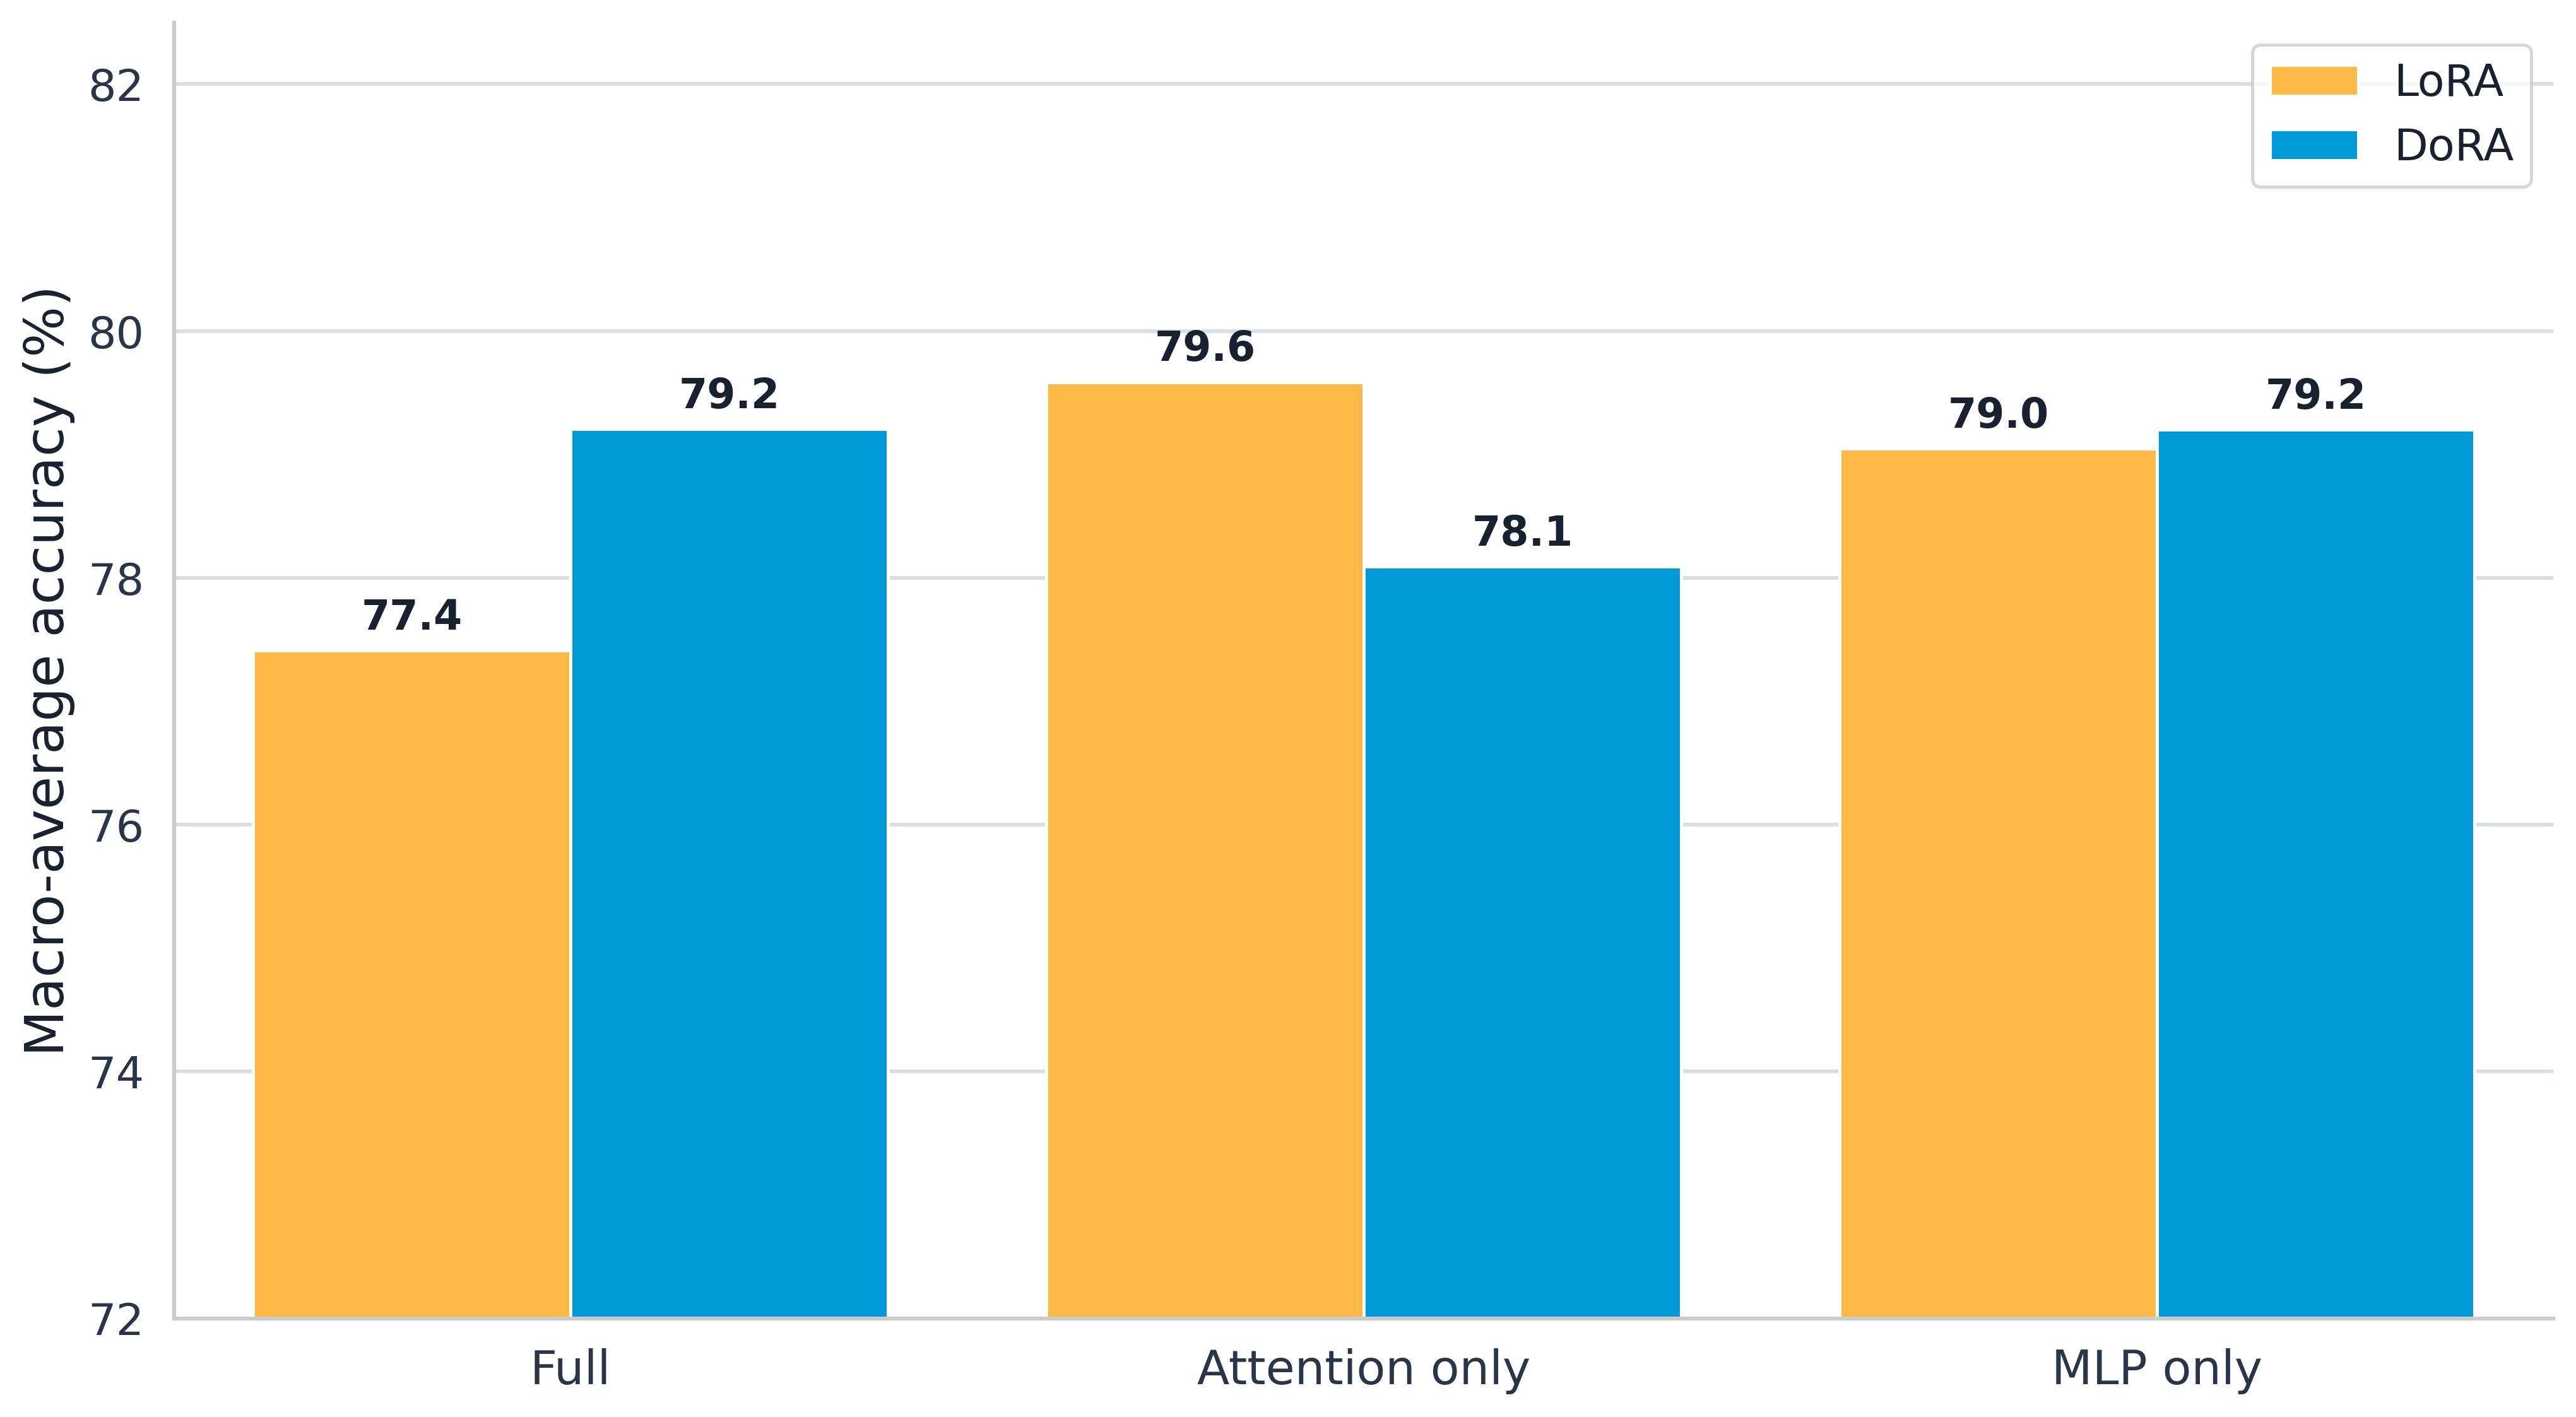
\includegraphics[width=0.98\linewidth]{fig1_macro_grouped.png}
\tightcaption{Full-scope \dora{} improves macro accuracy from 77.4\% to 79.2\%. Attention-only \dora{} does not improve over its matched \lora{} baseline.}

\vspace{0.8ex}
\small
\begin{center}
\begin{tabular}{lrrr}
\toprule
\textbf{Scope} & \textbf{\lora{} macro} & \textbf{\dora{} macro} & \textbf{Delta} \\
\midrule
Full & 77.41\% & \textbf{79.20\%} & \textbf{+1.79} \\
Attention only & \textbf{79.59\%} & 78.09\% & -1.50 \\
MLP only & 79.05\% & \textbf{79.20\%} & +0.15 \\
\bottomrule
\end{tabular}
\end{center}
\normalsize
\end{block}

\begin{block}{Where Does DoRA Help?}
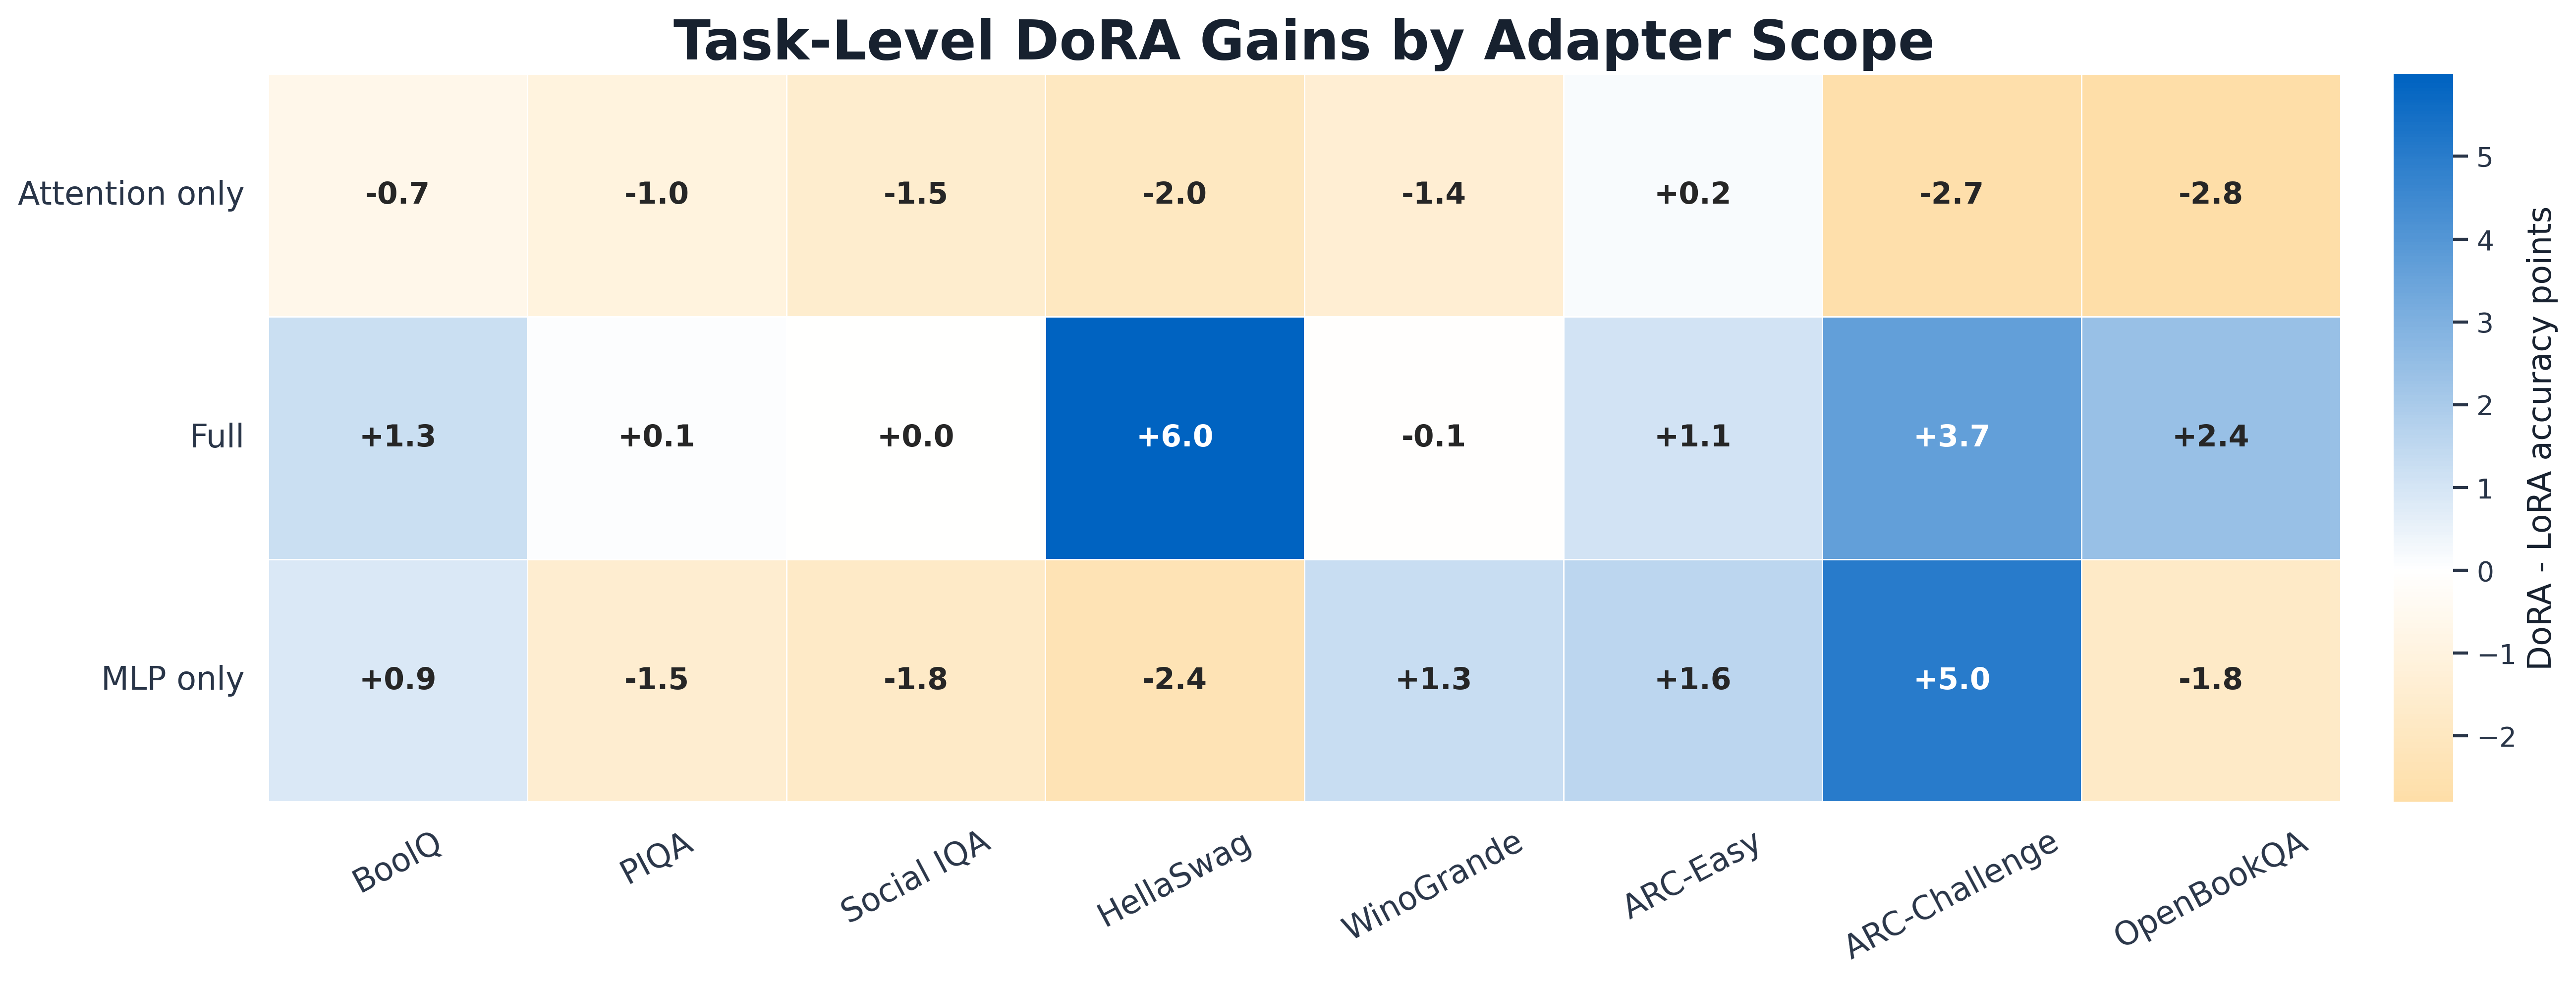
\includegraphics[width=0.98\linewidth]{fig3_dora_gains.png}
\tightcaption{Task-level \dora{} minus \lora{} gains. Full-scope \dora{} improves 6/8 tasks, ties Social IQA, and slightly loses on WinoGrande.}
\resultnote{Largest full-scope gains}{HellaSwag +6.0, ARC-Challenge +3.7, OpenBookQA +2.4 accuracy points.}
\end{block}

\end{column}

\separatorcolumn

% ====================
% Column 3
% ====================

\begin{column}{\colwidth}

\begin{block}{Official Reference Context}
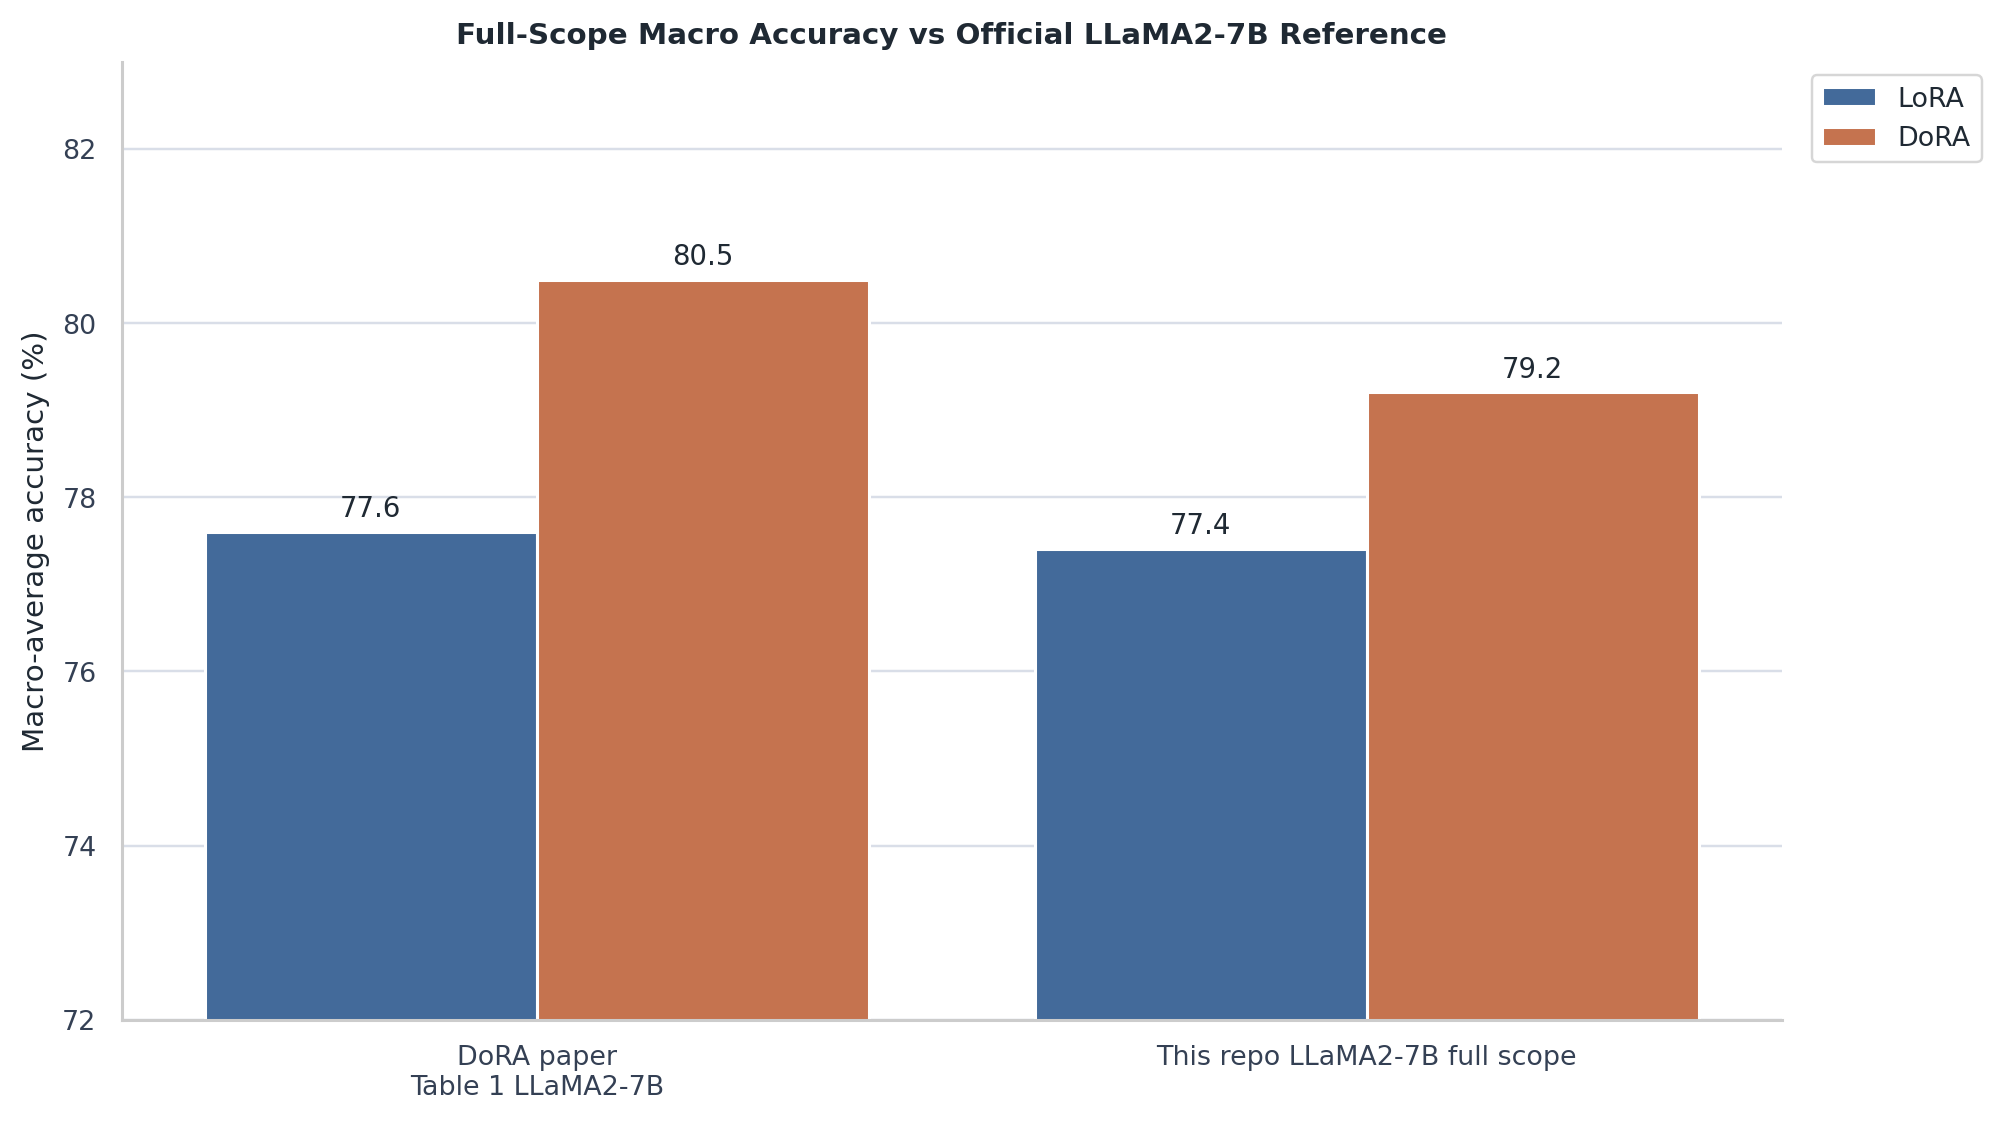
\includegraphics[width=0.98\linewidth]{fig5_official_comparison.png}
\tightcaption{Our result matches the paper's direction of improvement, but the absolute \dora{} score remains below the official LLaMA2-7B reference.}
\end{block}

\begin{exampleblock}{Interpretation}
\begin{itemize}
  \item The main paper-level claim \textbf{partially reproduced}: full-scope \dora{} beat full-scope \lora{}.
  \item Gains were not uniform across isolated module groups.
  \item Attention-only \dora{} underperformed attention-only \lora{} on 7/8 tasks.
  \item MLP-only \dora{} was roughly tied overall: ARC gains were offset by drops on PIQA, Social IQA, HellaSwag, and OpenBookQA.
  \item Best hypothesis: \dora{}'s magnitude/direction split works best when attention and MLP transformations can adapt together.
\end{itemize}
\end{exampleblock}

\begin{block}{Conclusion \& Future Work}
\heading{Takeaways}
\begin{itemize}
  \item Full-scope \dora{} improved macro-average accuracy by \textbf{+1.79 points}.
  \item The reproduction supports the qualitative value of weight-decomposed low-rank adaptation.
  \item The ablation adds a caution: applying \dora{} narrowly can remove the benefit.
\end{itemize}

\heading{Next steps}
\begin{itemize}
  \item Train on the full \texttt{commonsense\_170k.json} dataset.
  \item Repeat all six conditions across multiple random seeds.
  \item Test Llama-3-8B and larger Llama-family models.
  \item Add parameter-count, GPU-memory, and wall-clock comparisons.
  \item Analyze wrong answers by task, especially HellaSwag, ARC-Challenge, and OpenBookQA.
\end{itemize}
\end{block}

\begin{block}{References}
\tiny
\setbeamertemplate{bibliography item}[text]
\nocite{nvlabsdora,transformers}
\bibliographystyle{plain}
\bibliography{refs}
\end{block}

\end{column}

\separatorcolumn
\end{columns}
\end{frame}

\end{document}
